% Options for packages loaded elsewhere
\PassOptionsToPackage{unicode}{hyperref}
\PassOptionsToPackage{hyphens}{url}
\PassOptionsToPackage{dvipsnames,svgnames,x11names}{xcolor}
%
\documentclass[
  11pt,
  a4paper,
]{scrartcl}
\title{Homework 3 Report}
\usepackage{etoolbox}
\makeatletter
\providecommand{\subtitle}[1]{% add subtitle to \maketitle
  \apptocmd{\@title}{\par {\large #1 \par}}{}{}
}
\makeatother
\subtitle{Classification of liver malfunction severity (LDA)}
\author{Ian Effendi \textbackslash{}
\href{mailto:iae2784@rit.edu}{\nolinkurl{iae2784@rit.edu}}}
\date{October 12, 2021}

\usepackage{amsmath,amssymb}
\usepackage{lmodern}
\usepackage{iftex}
\ifPDFTeX
  \usepackage[T1]{fontenc}
  \usepackage[utf8]{inputenc}
  \usepackage{textcomp} % provide euro and other symbols
\else % if luatex or xetex
  \usepackage{unicode-math}
  \defaultfontfeatures{Scale=MatchLowercase}
  \defaultfontfeatures[\rmfamily]{Ligatures=TeX,Scale=1}
\fi
% Use upquote if available, for straight quotes in verbatim environments
\IfFileExists{upquote.sty}{\usepackage{upquote}}{}
\IfFileExists{microtype.sty}{% use microtype if available
  \usepackage[]{microtype}
  \UseMicrotypeSet[protrusion]{basicmath} % disable protrusion for tt fonts
}{}
\makeatletter
\@ifundefined{KOMAClassName}{% if non-KOMA class
  \IfFileExists{parskip.sty}{%
    \usepackage{parskip}
  }{% else
    \setlength{\parindent}{0pt}
    \setlength{\parskip}{6pt plus 2pt minus 1pt}}
}{% if KOMA class
  \KOMAoptions{parskip=half}}
\makeatother
\usepackage{xcolor}
\IfFileExists{xurl.sty}{\usepackage{xurl}}{} % add URL line breaks if available
\IfFileExists{bookmark.sty}{\usepackage{bookmark}}{\usepackage{hyperref}}
\hypersetup{
  pdftitle={Homework 3 Report},
  pdfauthor={Ian Effendi \textbackslash{} iae2784@rit.edu},
  colorlinks=true,
  linkcolor={Maroon},
  filecolor={Maroon},
  citecolor={Blue},
  urlcolor={violet},
  pdfcreator={LaTeX via pandoc}}
\urlstyle{same} % disable monospaced font for URLs
\usepackage[margin=1in,heightrounded]{geometry}
\usepackage{color}
\usepackage{fancyvrb}
\newcommand{\VerbBar}{|}
\newcommand{\VERB}{\Verb[commandchars=\\\{\}]}
\DefineVerbatimEnvironment{Highlighting}{Verbatim}{commandchars=\\\{\}}
% Add ',fontsize=\small' for more characters per line
\usepackage{framed}
\definecolor{shadecolor}{RGB}{248,248,248}
\newenvironment{Shaded}{\begin{snugshade}}{\end{snugshade}}
\newcommand{\AlertTok}[1]{\textcolor[rgb]{0.94,0.16,0.16}{#1}}
\newcommand{\AnnotationTok}[1]{\textcolor[rgb]{0.56,0.35,0.01}{\textbf{\textit{#1}}}}
\newcommand{\AttributeTok}[1]{\textcolor[rgb]{0.77,0.63,0.00}{#1}}
\newcommand{\BaseNTok}[1]{\textcolor[rgb]{0.00,0.00,0.81}{#1}}
\newcommand{\BuiltInTok}[1]{#1}
\newcommand{\CharTok}[1]{\textcolor[rgb]{0.31,0.60,0.02}{#1}}
\newcommand{\CommentTok}[1]{\textcolor[rgb]{0.56,0.35,0.01}{\textit{#1}}}
\newcommand{\CommentVarTok}[1]{\textcolor[rgb]{0.56,0.35,0.01}{\textbf{\textit{#1}}}}
\newcommand{\ConstantTok}[1]{\textcolor[rgb]{0.00,0.00,0.00}{#1}}
\newcommand{\ControlFlowTok}[1]{\textcolor[rgb]{0.13,0.29,0.53}{\textbf{#1}}}
\newcommand{\DataTypeTok}[1]{\textcolor[rgb]{0.13,0.29,0.53}{#1}}
\newcommand{\DecValTok}[1]{\textcolor[rgb]{0.00,0.00,0.81}{#1}}
\newcommand{\DocumentationTok}[1]{\textcolor[rgb]{0.56,0.35,0.01}{\textbf{\textit{#1}}}}
\newcommand{\ErrorTok}[1]{\textcolor[rgb]{0.64,0.00,0.00}{\textbf{#1}}}
\newcommand{\ExtensionTok}[1]{#1}
\newcommand{\FloatTok}[1]{\textcolor[rgb]{0.00,0.00,0.81}{#1}}
\newcommand{\FunctionTok}[1]{\textcolor[rgb]{0.00,0.00,0.00}{#1}}
\newcommand{\ImportTok}[1]{#1}
\newcommand{\InformationTok}[1]{\textcolor[rgb]{0.56,0.35,0.01}{\textbf{\textit{#1}}}}
\newcommand{\KeywordTok}[1]{\textcolor[rgb]{0.13,0.29,0.53}{\textbf{#1}}}
\newcommand{\NormalTok}[1]{#1}
\newcommand{\OperatorTok}[1]{\textcolor[rgb]{0.81,0.36,0.00}{\textbf{#1}}}
\newcommand{\OtherTok}[1]{\textcolor[rgb]{0.56,0.35,0.01}{#1}}
\newcommand{\PreprocessorTok}[1]{\textcolor[rgb]{0.56,0.35,0.01}{\textit{#1}}}
\newcommand{\RegionMarkerTok}[1]{#1}
\newcommand{\SpecialCharTok}[1]{\textcolor[rgb]{0.00,0.00,0.00}{#1}}
\newcommand{\SpecialStringTok}[1]{\textcolor[rgb]{0.31,0.60,0.02}{#1}}
\newcommand{\StringTok}[1]{\textcolor[rgb]{0.31,0.60,0.02}{#1}}
\newcommand{\VariableTok}[1]{\textcolor[rgb]{0.00,0.00,0.00}{#1}}
\newcommand{\VerbatimStringTok}[1]{\textcolor[rgb]{0.31,0.60,0.02}{#1}}
\newcommand{\WarningTok}[1]{\textcolor[rgb]{0.56,0.35,0.01}{\textbf{\textit{#1}}}}
\usepackage{graphicx}
\makeatletter
\def\maxwidth{\ifdim\Gin@nat@width>\linewidth\linewidth\else\Gin@nat@width\fi}
\def\maxheight{\ifdim\Gin@nat@height>\textheight\textheight\else\Gin@nat@height\fi}
\makeatother
% Scale images if necessary, so that they will not overflow the page
% margins by default, and it is still possible to overwrite the defaults
% using explicit options in \includegraphics[width, height, ...]{}
\setkeys{Gin}{width=\maxwidth,height=\maxheight,keepaspectratio}
% Set default figure placement to htbp
\makeatletter
\def\fps@figure{htbp}
\makeatother
\setlength{\emergencystretch}{3em} % prevent overfull lines
\providecommand{\tightlist}{%
  \setlength{\itemsep}{0pt}\setlength{\parskip}{0pt}}
\setcounter{secnumdepth}{-\maxdimen} % remove section numbering
\ifLuaTeX
  \usepackage{selnolig}  % disable illegal ligatures
\fi

\begin{document}
\maketitle

{
\hypersetup{linkcolor=blue}
\setcounter{tocdepth}{3}
\tableofcontents
}
\hypertarget{certification}{%
\subsection{Certification}\label{certification}}

\begin{quote}
I certify that I indeed finished reading Ch. 4 from \emph{An
Introduction to Statistical Learning}, by James Gareth, Daniela Witten,
Trevor Hastie, Robert Tibshirani.
\end{quote}

\hypertarget{overview}{%
\subsection{Overview}\label{overview}}

In this assignment we will:

\begin{itemize}
\tightlist
\item
  Perform exploratory data analysis (\emph{EDA}) on the dataset.
\item
  Fit and analyze a linear discriminant analysis (\emph{LDA}) model on
  the dataset.
\item
  Perform multiple cross-validation tasks at different \(k\)-fold values
  (\(k=3,\,k=10\)).
\end{itemize}

\hypertarget{elt}{%
\subsection{ELT}\label{elt}}

\emph{Much of the \textbf{extract}, \textbf{load}, and
\textbf{transform} (\textbf{ELT}) process from the previous report has
been revised for this assignment. Notably, a \texttt{make.dataset()}
function streamlines the process of parsing the source
\texttt{Liver.txt} file into a compatible \texttt{data.frame}.}

\begin{Shaded}
\begin{Highlighting}[]
\CommentTok{\# Import the dataset as variable called "Liver".}
\FunctionTok{invisible}\NormalTok{(}\FunctionTok{setup.analysis}\NormalTok{(}\AttributeTok{target =} \StringTok{"Liver"}\NormalTok{))}
\end{Highlighting}
\end{Shaded}

\begin{verbatim}
## Use cached dataset? TRUE
\end{verbatim}

\begin{verbatim}
## 'Liver' exists.
\end{verbatim}

\begin{verbatim}
## Importing dataset...
\end{verbatim}

\begin{verbatim}
## Parsing dataset from local file...
\end{verbatim}

\begin{verbatim}
## Reading dataset from compressed cache file...
\end{verbatim}

\begin{verbatim}
## Done.
\end{verbatim}

\begin{verbatim}
## Dataset imported.
\end{verbatim}

\begin{verbatim}
## Registered target dataset to global environment. Access using 'Liver'.
\end{verbatim}

\begin{verbatim}
## Use 'Liver' to access underlying tbl_df.
\end{verbatim}

\begin{verbatim}
## Dataset of type: 'tbl_df/tbl/data.frame'.
\end{verbatim}

\begin{verbatim}
## tibble [345 x 7] (S3: tbl_df/tbl/data.frame)
##  $ blood.1 : int [1:345] 85 85 86 91 87 98 88 88 92 90 ...
##  $ blood.2 : int [1:345] 92 64 54 78 70 55 62 67 54 60 ...
##  $ blood.3 : int [1:345] 45 59 33 34 12 13 20 21 22 25 ...
##  $ blood.4 : int [1:345] 27 32 16 24 28 17 17 11 20 19 ...
##  $ blood.5 : int [1:345] 31 23 54 36 10 17 9 11 7 5 ...
##  $ drinks  : num [1:345] 0 0 0 0 0 0 0.5 0.5 0.5 0.5 ...
##  $ severity: Factor w/ 2 levels "Not Severe","Severe": 2 1 1 1 1 1 2 2 2 2 ...
\end{verbatim}

The \texttt{setup.analysis()} function imports a dataset into the global
environment with the name provided to the \texttt{target\ =} argument.

\hypertarget{eda}{%
\subsection{EDA}\label{eda}}

\emph{This section reviews the \texttt{Liver} dataset. In an improvement
over the previous report, it now incorporates an assessment of feature
correlations.}

\hypertarget{response-encoding}{%
\subsubsection{Response Encoding}\label{response-encoding}}

\begin{Shaded}
\begin{Highlighting}[]
\CommentTok{\# Recode the response.}
\NormalTok{liver }\OtherTok{\textless{}{-}}\NormalTok{ Liver }\SpecialCharTok{\%\textgreater{}\%} \FunctionTok{make.response}\NormalTok{()}
\FunctionTok{summary}\NormalTok{(liver)}
\end{Highlighting}
\end{Shaded}

\begin{verbatim}
##     blood.1         blood.2         blood.3     
##  Min.   : 65.0   Min.   : 23.0   Min.   :  4.0  
##  1st Qu.: 87.0   1st Qu.: 57.0   1st Qu.: 19.0  
##  Median : 90.0   Median : 67.0   Median : 26.0  
##  Mean   : 90.2   Mean   : 69.9   Mean   : 30.4  
##  3rd Qu.: 93.0   3rd Qu.: 80.0   3rd Qu.: 34.0  
##  Max.   :103.0   Max.   :138.0   Max.   :155.0  
##     blood.4        blood.5          drinks     
##  Min.   : 5.0   Min.   :  5.0   Min.   : 0.00  
##  1st Qu.:19.0   1st Qu.: 15.0   1st Qu.: 0.50  
##  Median :23.0   Median : 25.0   Median : 3.00  
##  Mean   :24.6   Mean   : 38.3   Mean   : 3.46  
##  3rd Qu.:27.0   3rd Qu.: 46.0   3rd Qu.: 6.00  
##  Max.   :82.0   Max.   :297.0   Max.   :20.00  
##        severity  
##  Not Severe:200  
##  Severe    :145  
##                  
##                  
##                  
## 
\end{verbatim}

\begin{Shaded}
\begin{Highlighting}[]
\NormalTok{truth }\OtherTok{\textless{}{-}}\NormalTok{ (liver}\SpecialCharTok{$}\NormalTok{severity }\SpecialCharTok{==} \StringTok{"Severe"}\NormalTok{)}
\end{Highlighting}
\end{Shaded}

\newpage

\hypertarget{feature-correlations}{%
\subsubsection{Feature Correlations}\label{feature-correlations}}

\begin{Shaded}
\begin{Highlighting}[]
\NormalTok{liver.info }\OtherTok{\textless{}{-}} \FunctionTok{analysis.eda}\NormalTok{(Liver, truth)}
\FunctionTok{summary}\NormalTok{(liver.info)}
\end{Highlighting}
\end{Shaded}

\begin{verbatim}
##  n_samples n_features 
##        345          7 
## Label counts: 
##   pos   neg total 
##   145   200   345 
## Class prior probabilities: 
##    pos    neg 
## 0.4203 0.5797
\end{verbatim}

\begin{Shaded}
\begin{Highlighting}[]
\CommentTok{\# Plot using corrplot::corrplot wrapper.}
\NormalTok{liver.corrplot }\OtherTok{\textless{}{-}} \FunctionTok{corr.plot}\NormalTok{(}
\NormalTok{  liver, }\AttributeTok{sig.level =} \FloatTok{0.05}\NormalTok{, }\AttributeTok{insig =} \StringTok{"blank"}\NormalTok{,}
  \AttributeTok{title =} \StringTok{"Correlation Plot"}\NormalTok{,}
  \AttributeTok{mar =} \FunctionTok{c}\NormalTok{(}\DecValTok{1}\NormalTok{,}\DecValTok{1}\NormalTok{,}\DecValTok{2}\NormalTok{,}\DecValTok{1}\NormalTok{)}
\NormalTok{)}
\end{Highlighting}
\end{Shaded}

\begin{center}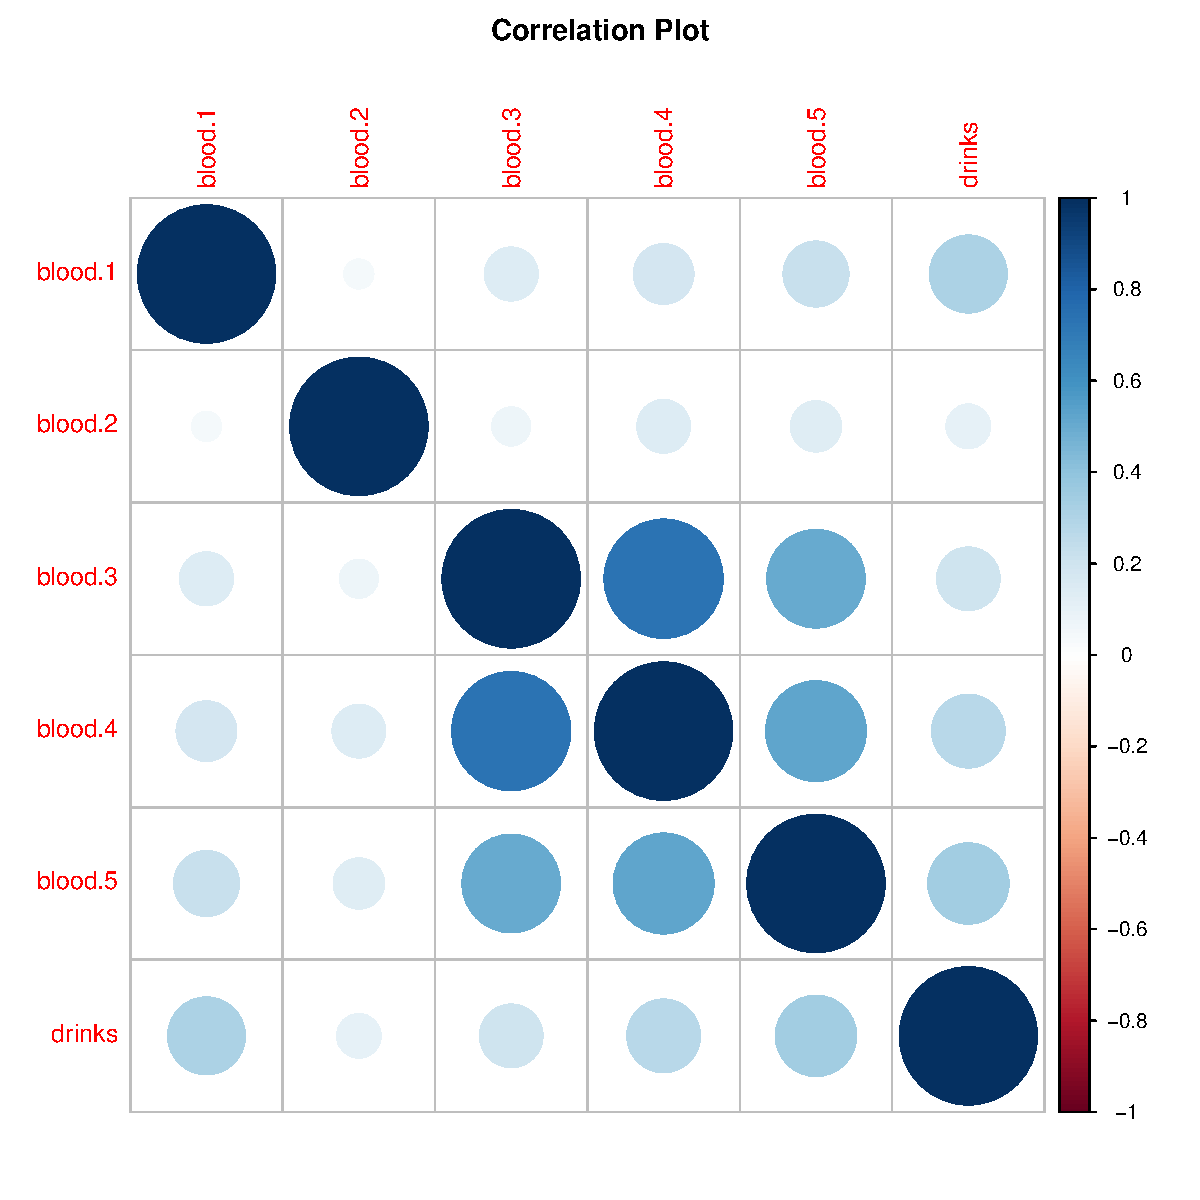
\includegraphics{figure/analysis-eda-corrplot-1} \end{center}

The data behind the above correlation plot is provided below:

\begin{verbatim}
## Feature correlation matrix: 
##         blood.1 blood.2 blood.3 blood.4 blood.5 drinks
## blood.1  1.0000 0.04410 0.14770  0.1878  0.2223 0.3127
## blood.2  0.0441 1.00000 0.07621  0.1461  0.1331 0.1008
## blood.3  0.1477 0.07621 1.00000  0.7397  0.5034 0.2068
## blood.4  0.1878 0.14606 0.73967  1.0000  0.5276 0.2796
## blood.5  0.2223 0.13314 0.50344  0.5276  1.0000 0.3412
## drinks   0.3127 0.10080 0.20685  0.2796  0.3412 1.0000
\end{verbatim}

\hypertarget{model-analysis}{%
\subsection{Model Analysis}\label{model-analysis}}

Models will be tracked using a named list \texttt{MODELS}:

\begin{Shaded}
\begin{Highlighting}[]
\CommentTok{\# Create a global \textasciigrave{}models\textasciigrave{} variable to keep track of models.}
\NormalTok{MODELS }\OtherTok{\textless{}\textless{}{-}} \FunctionTok{list}\NormalTok{()}
\CommentTok{\# Also, declares a reusable formula.}
\NormalTok{.FORMULA }\OtherTok{\textless{}\textless{}{-}}\NormalTok{ severity }\SpecialCharTok{\textasciitilde{}}\NormalTok{ .}
\end{Highlighting}
\end{Shaded}

\hypertarget{baseline-model-analysis}{%
\subsubsection{Baseline Model Analysis}\label{baseline-model-analysis}}

\begin{Shaded}
\begin{Highlighting}[]
\CommentTok{\# Fit LDA with priors calculated from the input sample.}
\CommentTok{\# Equivalent to: MASS::lda(severity \textasciitilde{} ., data = liver)}
\CommentTok{\# We use \textasciigrave{}.\textasciigrave{} instead of \textasciigrave{}baseline\textasciigrave{} for ease of typing.}
\NormalTok{MODELS}\SpecialCharTok{$}\NormalTok{. }\OtherTok{\textless{}{-}} \FunctionTok{fit.model}\NormalTok{(}\FunctionTok{quote}\NormalTok{(liver), }\AttributeTok{algorithm =}\NormalTok{ lda, }\AttributeTok{formula =}\NormalTok{ .FORMULA)}

\CommentTok{\# Temporary variable \textasciigrave{}model\textasciigrave{} for current analysed model:}
\NormalTok{model }\OtherTok{\textless{}{-}}\NormalTok{ MODELS}\SpecialCharTok{$}\NormalTok{.}
\end{Highlighting}
\end{Shaded}

\begin{verbatim}
## Baseline LDA Summary:
## Call:
## lda(severity ~ ., data = liver)
## 
## Prior probabilities of groups:
## Not Severe     Severe 
##     0.5797     0.4203 
## 
## Group means:
##            blood.1 blood.2 blood.3 blood.4 blood.5 drinks
## Not Severe   89.81   68.34   29.82   25.99   43.17  3.393
## Severe       90.63   71.98   31.21   22.79   31.54  3.541
## 
## Coefficients of linear discriminants:
##              LD1
## blood.1  0.08312
## blood.2  0.02263
## blood.3  0.05893
## blood.4 -0.11812
## blood.5 -0.01497
## drinks   0.06061
\end{verbatim}

\begin{verbatim}
## Baseline model error rate:
## 0.2957
## 
## Baseline misclassification table:
##             
##              Not Severe Severe
##   Not Severe        165     67
##   Severe             35     78
## 
## Total misclassified: 102
\end{verbatim}

\hypertarget{optimal-priors-for-total-error-rate}{%
\subsubsection{Optimal Priors (for Total Error
Rate)}\label{optimal-priors-for-total-error-rate}}

We can calculate the model that minimizes the total error rate while
explicitly setting the prior probability for the positive class. As a
reminder:

\[
p = P(\text{ Severe }),\, q = (1 - p) = P(\text{Not Severe})
\]

\begin{Shaded}
\begin{Highlighting}[]
\CommentTok{\# Prepare next analysis.}
\NormalTok{MODELS}\SpecialCharTok{$}\NormalTok{min\_error }\OtherTok{\textless{}{-}}\NormalTok{ LDA.ANALYSIS}\SpecialCharTok{$}\FunctionTok{calc.optimal.prior.error.rates}\NormalTok{(}
\NormalTok{  liver, truth,}
  \AttributeTok{formula =}\NormalTok{ severity }\SpecialCharTok{\textasciitilde{}}\NormalTok{ .,}
  \AttributeTok{from =} \FloatTok{0.001}\NormalTok{, }\AttributeTok{to =} \FloatTok{0.999}\NormalTok{, }\AttributeTok{m =} \DecValTok{25}\NormalTok{,}
  \AttributeTok{minimize\_cost =} \ConstantTok{FALSE}\NormalTok{, }\AttributeTok{penalty =} \DecValTok{10}
\NormalTok{)}
\end{Highlighting}
\end{Shaded}

\begin{verbatim}
## ---------------------------
## Finding optimal error rates with explicit priors.
## # Penalty factor applied to cost function: x10
## # Checking 25 pos class priors in range [0.001, 0.999]:
## tibble [25 x 2] (S3: tbl_df/tbl/data.frame)
##  $ p: num [1:25] 0.001 0.0426 0.0842 0.1258 0.1673 ...
##  $ q: num [1:25] 0.999 0.957 0.916 0.874 0.833 ...
## Summary of minimum error rate search:
## Min. total cost: 703 (Penalty = x10)
## Min. total error: 0.2899
## Min. total miss: 703
## Optimal q/p ratio: 1.39904038384646
## Optimal priors: p = 0.4168, q = 0.58317
## Summary: 
## tibble [1 x 7] (S3: tbl_df/tbl/data.frame)
##  $ p    : num 0.417
##  $ q    : num 0.583
##  $ fp   : int 67
##  $ fn   : int 33
##  $ miss : int 100
##  $ cost : num 703
##  $ error: num 0.29
## ---------------------------
\end{verbatim}

\begin{verbatim}
## ---------------------------
## Call:
## lda(severity ~ ., data = .data, prior = c(0.583166666666667, 
## 0.416833333333333))
## 
## Prior probabilities of groups:
## Not Severe     Severe 
##     0.5832     0.4168 
## 
## Group means:
##            blood.1 blood.2 blood.3 blood.4 blood.5 drinks
## Not Severe   89.81   68.34   29.82   25.99   43.17  3.393
## Severe       90.63   71.98   31.21   22.79   31.54  3.541
## 
## Coefficients of linear discriminants:
##              LD1
## blood.1  0.08312
## blood.2  0.02263
## blood.3  0.05893
## blood.4 -0.11812
## blood.5 -0.01497
## drinks   0.06061
## Total cost of misclassification (Penalty x10): 703.00
## Total error rate (100 misclassifications): 0.29
\end{verbatim}

\begin{verbatim}
##             
##              Not Severe Severe
##   Not Severe        167     67
##   Severe             33     78
## ---------------------------
\end{verbatim}

\hypertarget{optimal-priors-for-total-cost}{%
\subsubsection{Optimal Priors (for Total
Cost)}\label{optimal-priors-for-total-cost}}

Notice the current ``cost'' is a penalty factor of 10. The
\texttt{penalty} value is a ratio that can be used to scale how a
misclassification for the positive class affects the model.

We can also minimize our model based on the total cost. The following
plots summarize both scenarios:

\begin{center}\includegraphics{figure/analysis-lda-optimal-plot-1} \end{center}

\begin{center}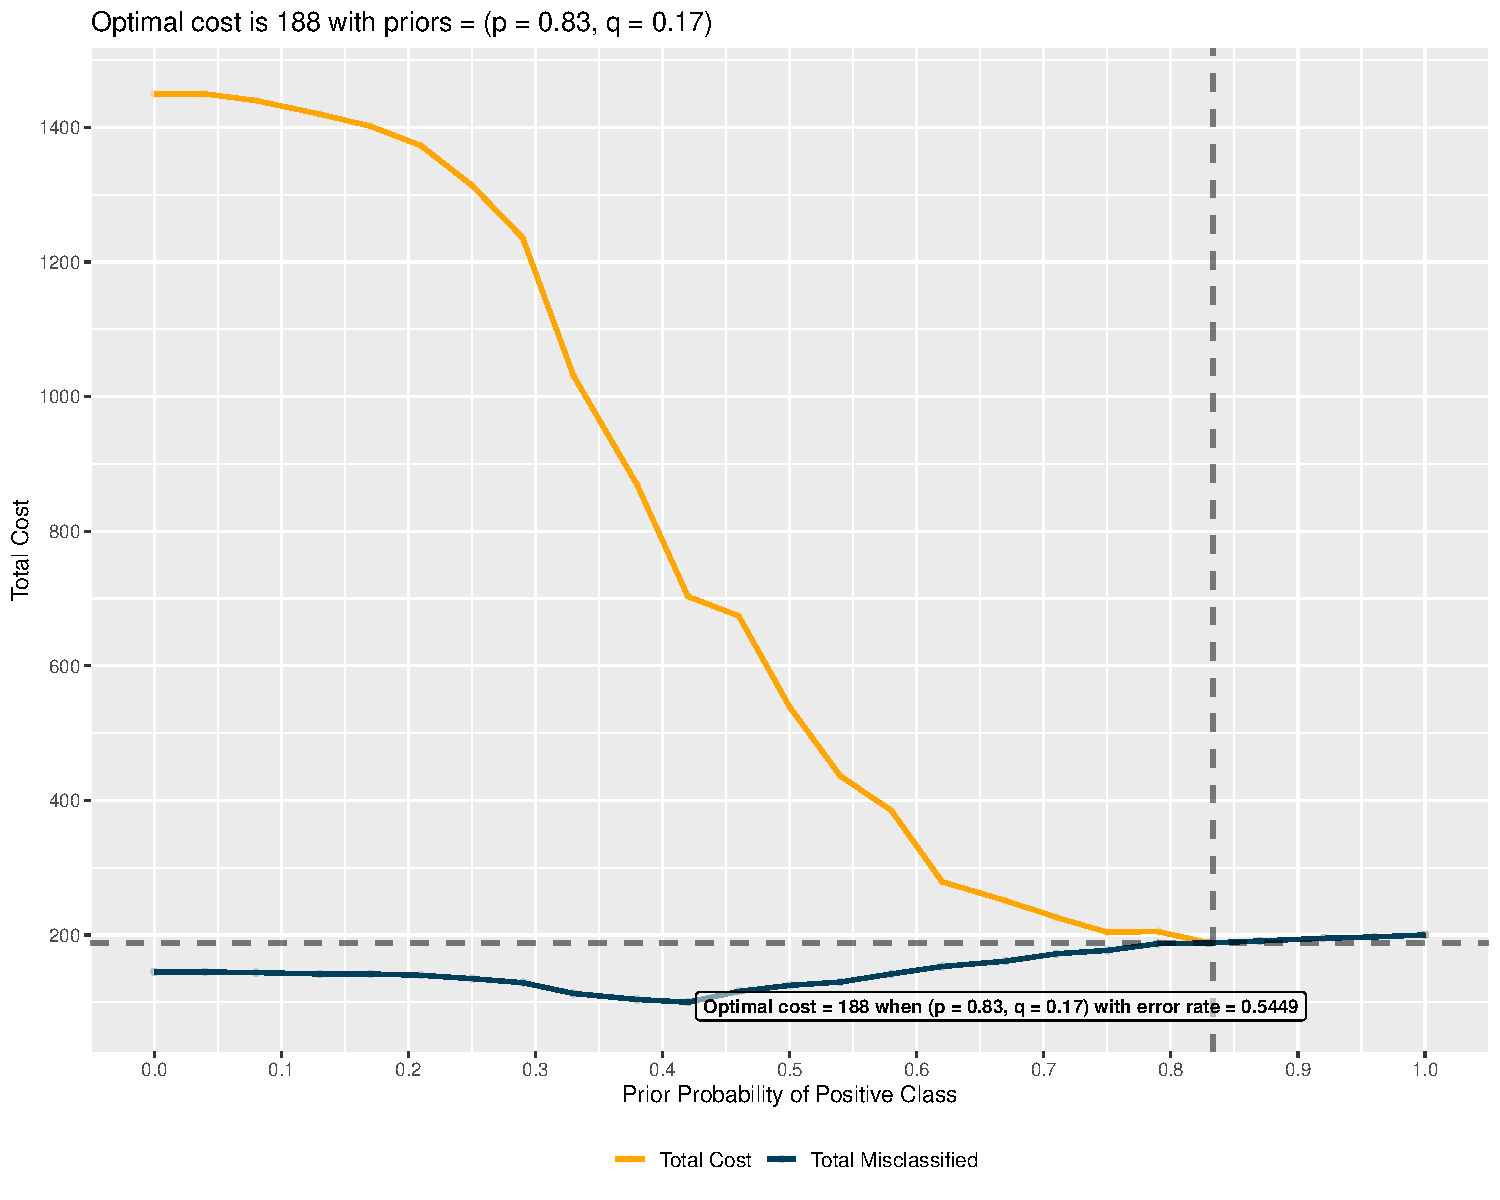
\includegraphics{figure/analysis-lda-optimal-plot-2} \end{center}

\begin{verbatim}
## ---------------------------
## Generating plot with priors of range [0.001, 0.999]
## # Searching for optimal values by minimizing total error rate.
## # Found optimal error rate from dataset: 0.2899
## # Total cost at optimal error rate: 703.00
## # Optimal priors for minimized total error rate: (p = 0.42, q = 0.58)
## # Cost calculated with penatly = 10
## ---------------------------
## ---------------------------
## Generating plot with priors of range [0.001, 0.999]
## # Searching for optimal values by minimizing total cost.
## # Found optimal cost from dataset: 188.00
## # Total error rate at optimal cost: 0.5449
## # Optimal priors for minimized cost: (p = 0.83, q = 0.17)
## # Cost calculated with penatly = 10
## ---------------------------
\end{verbatim}

\newpage

\hypertarget{cross-validation-analysis}{%
\subsection{Cross-Validation Analysis}\label{cross-validation-analysis}}

\begin{quote}
This section is a revision of the logistic regression CV. I was unable
to complete the LDA CV analysis but I had reworked this analysis from my
previous report in order to better understand how to accomplish the
assignment. I hope to submit a revision before solutions are released
for homework 3; the work is simply in progress.
\end{quote}

\hypertarget{fold-cv}{%
\subsubsection{10-fold CV}\label{fold-cv}}

\begin{verbatim}
## ---------------------------
## Performing 10-fold CV:
## # Samples: 345
## # Thresholds: 100
## # k folds: 10 || # rounds: 100
## ---------------------------
## tibble [100 x 4] (S3: tbl_df/tbl/data.frame)
##  $ total.err : num [1:100] 0.58 0.571 0.566 0.562 0.558 ...
##  $ ci.low    : num [1:100] 0.575 0.566 0.561 0.557 0.553 ...
##  $ ci.high   : num [1:100] 0.585 0.576 0.571 0.567 0.563 ...
##  $ thresholds: num [1:100] 0 0.0101 0.0202 0.0303 0.0404 ...
## tibble [300 x 4] (S3: tbl_df/tbl/data.frame)
##  $ thresholds: num [1:300] 0 0 0 0.0101 0.0101 ...
##  $ category  : chr [1:300] "total.err" "ci.low" "ci.high" "total.err" ...
##  $ error     : num [1:300] 0.58 0.575 0.585 0.571 0.566 ...
##  $ linetype  : logi [1:300] TRUE FALSE FALSE TRUE FALSE FALSE ...
## ---------------------------
## Calculating 10-fold CV table:
## # Samples: 345
## # Threshold: 1
## # k folds: 10 || # rounds: 100
## ---------------------------
##                       Length Class  Mode   
## results                  2   -none- list   
## plot                     2   -none- list   
## optimal_threshold        1   -none- numeric
## confusion_mat         4000   -none- numeric
## confusion_mat_summary    2   -none- list
\end{verbatim}

\begin{center}\includegraphics{figure/analysis-glm-10cv-plot-1} \end{center}

\begin{verbatim}
## $plot
## 
## $optimal_threshold
## [1] 0.5253
\end{verbatim}

\begin{verbatim}
## Optimal threshold: 0.525252525252525
## $mean
##        [,1]  [,2]
## [1,] 167.61 73.08
## [2,]  32.39 71.92
## 
## $sterr
##        [,1]   [,2]
## [1,] 0.1974 0.2038
## [2,] 0.1974 0.2038
\end{verbatim}

\newpage

\hypertarget{fold-cv-1}{%
\subsubsection{3-fold CV}\label{fold-cv-1}}

\begin{verbatim}
## ---------------------------
## Performing 3-fold CV:
## # Samples: 345
## # Thresholds: 100
## # k folds: 3 || # rounds: 100
## ---------------------------
## tibble [100 x 4] (S3: tbl_df/tbl/data.frame)
##  $ total.err : num [1:100] 0.58 0.57 0.565 0.561 0.558 ...
##  $ ci.low    : num [1:100] 0.575 0.566 0.561 0.556 0.553 ...
##  $ ci.high   : num [1:100] 0.584 0.575 0.57 0.565 0.562 ...
##  $ thresholds: num [1:100] 0 0.0101 0.0202 0.0303 0.0404 ...
## tibble [300 x 4] (S3: tbl_df/tbl/data.frame)
##  $ thresholds: num [1:300] 0 0 0 0.0101 0.0101 ...
##  $ category  : chr [1:300] "total.err" "ci.low" "ci.high" "total.err" ...
##  $ error     : num [1:300] 0.58 0.575 0.584 0.57 0.566 ...
##  $ linetype  : logi [1:300] TRUE FALSE FALSE TRUE FALSE FALSE ...
## ---------------------------
## Calculating 3-fold CV table:
## # Samples: 345
## # Threshold: 1
## # k folds: 3 || # rounds: 100
## ---------------------------
##                       Length Class  Mode   
## results                  2   -none- list   
## plot                     2   -none- list   
## optimal_threshold        1   -none- numeric
## confusion_mat         1200   -none- numeric
## confusion_mat_summary    2   -none- list
\end{verbatim}

\begin{center}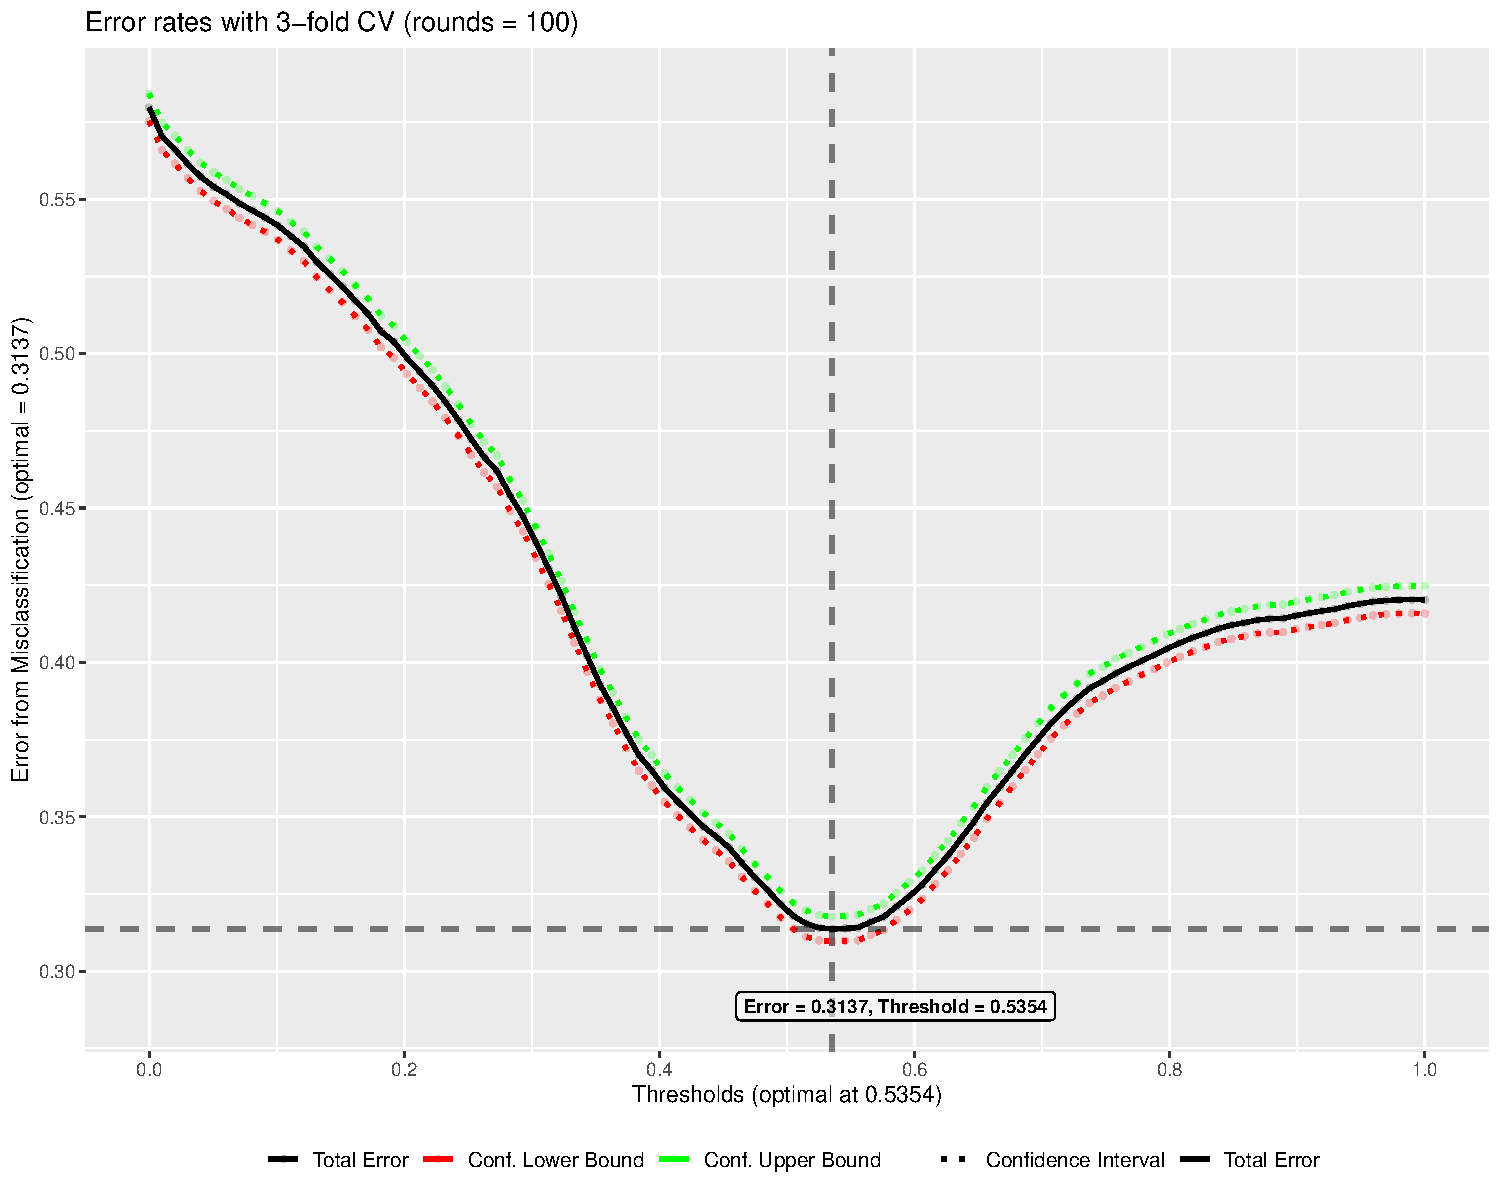
\includegraphics{figure/analysis-glm-3cv-plot-1} \end{center}

\begin{verbatim}
## $plot
## 
## $optimal_threshold
## [1] 0.5354
\end{verbatim}

\begin{verbatim}
## Optimal threshold: 0.535353535353535
## $mean
##        [,1]  [,2]
## [1,] 168.56 76.46
## [2,]  31.44 68.54
## 
## $sterr
##        [,1]   [,2]
## [1,] 0.3436 0.3301
## [2,] 0.3436 0.3301
\end{verbatim}

\newpage

\hypertarget{session-information}{%
\subsection{Session Information}\label{session-information}}

\emph{This document was generated from an
\href{http://rmarkdown.rstudio.com}{R Markdown} Notebook (See the
\texttt{vignettes/HW3\_report.Rmd} in the project's sub-directory). The
setup chunk for this document sets the root directory to the project
root directory using the \texttt{here} package; all file paths are
relative to the project root.}

\begin{verbatim}
## R version 4.1.1 (2021-08-10)
## Platform: x86_64-w64-mingw32/x64 (64-bit)
## Running under: Windows 10 x64 (build 19043)
## 
## Matrix products: default
## 
## locale:
## [1] LC_COLLATE=English_United States.1252 
## [2] LC_CTYPE=English_United States.1252   
## [3] LC_MONETARY=English_United States.1252
## [4] LC_NUMERIC=C                          
## [5] LC_TIME=English_United States.1252    
## 
## attached base packages:
## [1] stats     graphics  grDevices datasets  utils    
## [6] methods   base     
## 
## other attached packages:
##  [1] dplyr_1.0.7    tidyr_1.1.4    tibble_3.1.5  
##  [4] forcats_0.5.1  ggplot2_3.3.5  foreach_1.5.1 
##  [7] magrittr_2.0.1 MASS_7.3-54    mime_0.12     
## [10] markdown_1.1   rmarkdown_2.11 knitr_1.36    
## 
## loaded via a namespace (and not attached):
##  [1] highr_0.9        jquerylib_0.1.4  compiler_4.1.1  
##  [4] pillar_1.6.3     iterators_1.0.13 tools_4.1.1     
##  [7] corrplot_0.90    bit_4.0.4        digest_0.6.28   
## [10] jsonlite_1.7.2   evaluate_0.14    lifecycle_1.0.1 
## [13] gtable_0.3.0     pkgconfig_2.0.3  rlang_0.4.11    
## [16] cli_3.0.1        rstudioapi_0.13  yaml_2.2.1      
## [19] xfun_0.26        fastmap_1.1.0    stringr_1.4.0   
## [22] withr_2.4.2      hms_1.1.1        generics_0.1.0  
## [25] vctrs_0.3.8      bit64_4.0.5      rprojroot_2.0.2 
## [28] grid_4.1.1       tidyselect_1.1.1 glue_1.4.2      
## [31] here_1.0.1       R6_2.5.1         fansi_0.5.0     
## [34] vroom_1.5.5      farver_2.1.0     tzdb_0.1.2      
## [37] readr_2.0.2      purrr_0.3.4      scales_1.1.1    
## [40] codetools_0.2-18 htmltools_0.5.2  ellipsis_0.3.2  
## [43] colorspace_2.0-2 renv_0.14.0      labeling_0.4.2  
## [46] utf8_1.2.2       stringi_1.7.5    munsell_0.5.0   
## [49] crayon_1.4.1
\end{verbatim}

\end{document}
